\documentclass[a4paper,12pt]{article}
\usepackage[english]{babel}
\usepackage[utf8]{inputenc}
\usepackage{url}
\usepackage{graphicx}
\graphicspath{ {imgs/} }
\usepackage{floatrow}
\usepackage{amsfonts}
\usepackage{amssymb}
\usepackage{algorithm2e}

\usepackage{longtable}
\usepackage[acronym]{glossaries}
\usepackage{acro}

\usepackage{enumerate}% http://ctan.org/pkg/enumerate

\newcommand{\etal}{\textit{et al}. }
\newcommand{\ie}{\textit{i}.\textit{e}., }
\newcommand{\eg}{\textit{e}.\textit{g}. }
\newcommand{\etc}{\textit{etc}.}

% make paragraph start a new line instead of indent
\usepackage[parfill]{parskip}

%\usepackage[style=numeric,sortcites,backend=biber]{biblatex}
%\bibliography{test.bib}

% Glossary
%\makeglossaries
%\loadglsentries{acronyms}


%\newacronym{gcd}{GCD}{Greatest Common Divisor}

%%% to be done command
% set a to be done
\usepackage[textwidth=1.6cm]{todonotes}
\usepackage{xpatch}

\def\resetnamelevel#1{%
    \ifnum#1<1\let\thischaptername\relax\fi
    \ifnum#1<2\let\thissectionname\relax\fi
    \ifnum#1<3\let\thissubsectionname\relax\fi
    \ifnum#1<4\let\thissubsubsectionname\relax\fi
}\resetnamelevel{0}

\def\chaptername#1{\resetnamelevel{0}\def\thischaptername{#1}}
\def\sectionname#1{\resetnamelevel{1}\def\thissectionname{#1}}
\def\subsectionname#1{\resetnamelevel{2}\def\thissubsectionname{#1}}
\def\subsubsectionname#1{\resetnamelevel{3}\def\thissubsubsectionname{#1}}

\let\Chaptermark\chaptermark
\let\Sectionmark\sectionmark
\let\Subsectionmark\subsectionmark
\let\Subsubsectionmark\subsubsectionmark
\def\chaptermark#1{\chaptername{#1}\Chaptermark{#1}}
\def\sectionmark#1{\sectionname{#1}\Sectionmark{#1}}
\def\subsectionmark#1{\subsectionname{#1}\Subsectionmark{#1}}
\def\subsubsectionmark#1{\subsubsectionname{#1}\Subsubsectionmark{#1}}

\makeatletter
\newcommand\treeloc{%
    \ifx\thischaptername\relax%
        ??\@latex@warning{\textbackslash treeloc called outside of structure}
    \else
        \thischaptername%
        \ifx\thissectionname\relax%
        \else
            \ /\ \thissectionname%
            \ifx\thissubsectionname\relax%
            \else
                \ /\ \thissubsectionname%
                \ifx\thissubsubsectionname\relax%
                \else
                    \ /\ \thissubsubsectionname%
                \fi
            \fi
        \fi
    \fi
    }
\makeatother

\newcommand\tbd{%
    \todo[caption={TBD: \expandafter\treeloc}]{TBD}
}


%add an extra level of sections
\usepackage{titlesec}

\setcounter{secnumdepth}{4}

\titleformat{\paragraph}
{\normalfont\normalsize\bfseries}{\theparagraph}{1em}{}
\titlespacing*{\paragraph}
{0pt}{3.25ex plus 1ex minus .2ex}{1.5ex plus .2ex}


%Begining of the document
\begin{document}

\section*{Abstract}

%\tableofcontents

%abbrevation
\newacronym{DDT}{DDT}{Dynamic Driving Task}
\newacronym{OEDR}{OEDR}{Object and Event Detection and Response}
\newacronym{ODD}{ODD}{Operational Design Domain}
\newacronym{ADS}{ADS}{Active Safety Systems}
\newacronym{DARPA}{DARPA}{The Defense Advanced Research Projects Agency}
\newacronym{DL}{DL}{Deep Learning}
\newacronym{SVM}{SVM}{Support Vector Machine}
\newacronym{CNN}{CNN}{Convolutional Neural Network}
\newacronym{ILSVRC}{ILSVRC}{Large Scale Visual Recognition Challenge}
%\newacronym{}{}{}
%\newacronym{}{}{}
%\newacronym{}{}{}
%\newacronym{}{}{}
%\newacronym{}{}{}
%\newacronym{}{}{}
%\newacronym{}{}{}
%\printacronyms[include-classes=abbrev,name=Abbreviations]
%\printglossary[type=\acronymtype]




\section{Introduction}
\subsection{Motivation}
The autonomous vehicles (AVs) is the evolutionary direction of automobiles  due to its promising reliability and efficiency, as well as the underlying commercial profits. To gain a comprehensive perception of the driving environment is the very essential step for AVs. Object detection is one of the key challenges of perception. Thanks to the remarkable advancement of deep neural networks, great achievements have been make on 2D object detection, while 3D object detection is still underdeveloped. For example, according to the  KITTI Object Detection Benchmark\cite{Geiger2012CVPR}, the Average Precision (AP) of  top 10 2D car detection algorithms is over 90\% whereas best performance of 3D car detection is only 73.66\%. This gap results from the difficulty of adding the third dimension and the orientation of the 3D bounding box.

For AVs, 3D information of the surrounding vehicles is indispensable because it expresses the vehicle dimensions, locations and orientation in the real 3D environment, which is essential for AVs to perform planning and decision making. To find a safe and efficient route, the information of actual and potential movement, dimensions, and location of other vehicles is necessary. In order to perceive the movement, 3D localization,  orientation, and time are used to recover the velocity. The decision-making systems are more complicated and require more detailed 3D information, for example, the Bosch's Autonomous Emergency Braking systems (AEB) requires the distance to each part of a foregoing vehicle to decide whether or which level of brakes to apply.And it is common that some parts of the vehicle are occluded by other objects or truncated by the boundaries of the image. Thus, the exact location of each vehicle part and the visibility property of these parts are necessary.

Here we propose an approach that can simultaneously present the 3D dimensions, 3D localization, 3D bounding box orientation, 3D parts location, and parts visibility of a vehicle by giving a monocular image and all the 2D bounding boxes for vehicles. Figure 1 \tbd shows one output image example.



\subsection{Contributions}

The first contribution is that our approach can predict not only the 3D bounding box for each vehicle but also the 3D position of each vehicle part, even if these parts are occluded by other objects or truncated by the boundaries of the image. The foundation behind this is that vehicles are rigid objects and their geometric characteristics have a lot in common despite of the vehicle types. Therefore, these shared geometric characteristics serve as the priors which make it reasonable that each vehicle can to be expressed by a 3D artificial model along with a scaling vector. This 3D model is integrated by vehicle parts which are further encoded by characteristic points. Besides, we apply regression rather than detection to search and locate these characteristic points. By doing so, our approach can find all the rest of parts, as long as it ascertains the existence of the vehicle object and some parts. Therefore, even through some parts are invisible to the camera, our approach can still localize them. 

The second contribution is the proposed semi-automatic labelling process which generates additional labels to create a new dataset for our approach.  Deep neural networks are greedy for data. Manual labelling is time-consuming and error-prone, let alone it is infeasible to correctly label the very far vehicles or occluded parts in the image. Therefore, we eliminate the human labor to the extend where only the 3D models need to be labelled manually. Then the process automatically selects the best-matching model and projects this model into the real image to generate labels, \eg visibility and characteristic points.  Besides, this process can be easily generalized to other tasks, as long as they require 2D geometry information in the image coordinate and 3D geometry knowledge in the world coordinate.

The third contribution is the multi-task framework which includes a prediction neural network and a inference block. The network can simultaneously perform vehicle parts localization, visibility characterization, and template proximity prediction at high accuracy level and consequentially, the inference block performs the vehicle dimension estimation,  3D vehicle localization, and rotation recovery. All these tasks can be completed in real time, 0.02s per image, which makes it applicable to directly process the video sequence of the vehicle's front camera.

\section{Related Work}

\section{Background}
\subsection{A Short History of Autonomous Vehicles}

Autonomous Vehicles (a.k.a. Automated/Driverless/Unmanned/Robotic/Self-driving Vehicles) is a relatively vague concept to the public. Actually, it covers a continuum  from traditional fully human-driving automobiles to fully self-driving vehicles, as SAE classified in the Table \ref{figure:loa}.

\begin{table}[h]		
	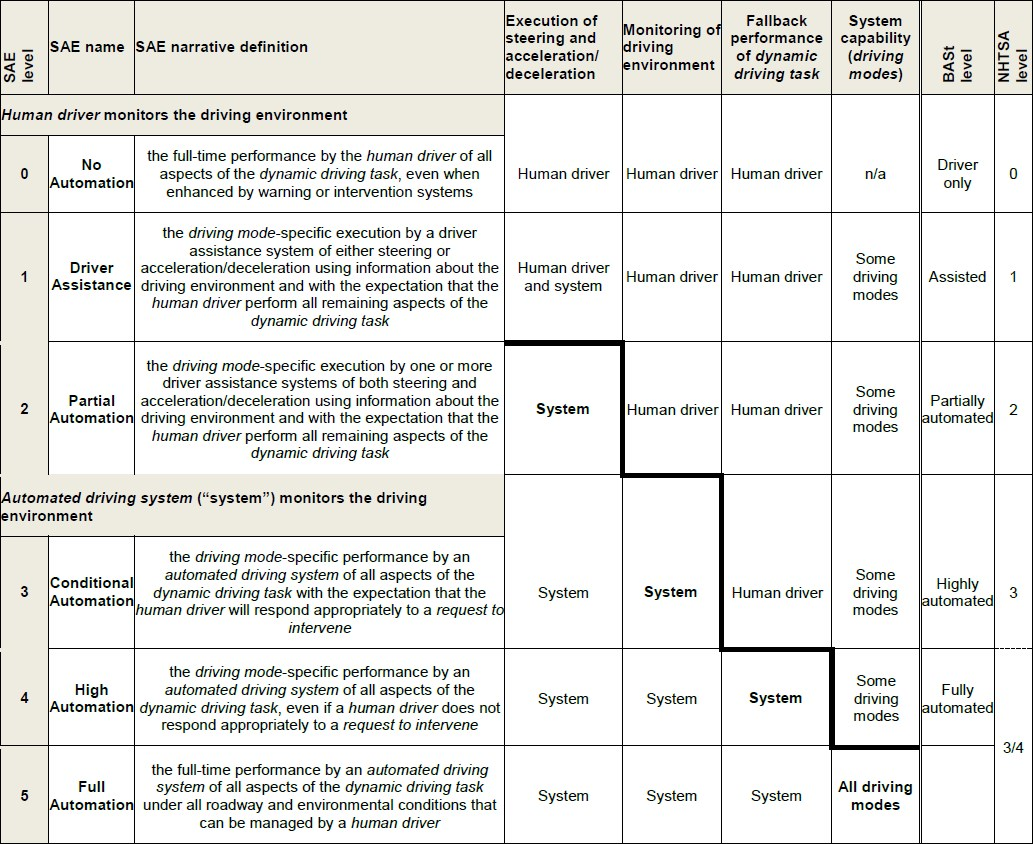
\includegraphics[width=1\textwidth]{Levels_of_Automation_2014.jpg}
	\caption{Summary of levels of driving automation\cite{J3016_201401}}
	\centering
	\label{figure:loa}
\end{table}

Contrary to the intuition, the idea of Autonomous Vehicles has a long history. The experiments of this fictional idea can be tracked back to 1920s and the technology behind it was radio control \cite{pawtc}. 

But the truly autonomous cars did not show up until 1980s, even though they could only move slowly on clear streets and required large human intervention. Mercedes-Benz demonstrated a robotic van based on saccadic vision \cite{schj}. The Autonomous Land Vehicle (ALV) project funded by The Defense Advanced Research Projects Agency (DARPA) cultivated automatic vehicles based on Computer Vision, LIDAR, and autonomous robotic control \cite{Kanade:1986:ALV:324634.325197}. Carnegie Mellon University initiatively applied neural network to control the vehicle \cite{NIPS1988_95}. 

In 1990s, huge progress was made.The VaMP from Daimler-Benz drove more than 1000 km, achieving the maximum speed of 130 km/h on a normal Pairs highway semi-autonomously \cite{schj}. The Navlab project in Carnegie Mellon University achieved a 5000 km  journey cross America with only 1.8\% human interventions \cite{nohand}. The ParkShuttle in Netherlands could autonomously navigate itself on a dedicated lane as an automated people mover \cite{parkshuttle}.In this decade, the experiments were mainly carried out in highway scenarios rather than urban scenes.

In 2000s, competitions promoted this technology a lot. One of the most famous is The DARPA Grand Challenge in U.S. who offered \$ 1 million for the first prize. In 2004, no vehicle completed the 241-km journey autonomously while 5 teams achieved this goal in 2005 \cite{Buehler2007}. And in Grand Challenge III 2007 , known as Urban Challenge, 6 vehicles  finished the event which was a 96 km urban route involving with traffic regulations and other vehicles \cite{Buehler2009}.

In 2010s,  Autonomous Driving Technology starts to take off. Numerous events and projects have been carried out and considerable companies, universities, and research centres have engaged into this field. Based on the progress made before, many autonomous vehicle systems are being tested or even brought into production.  Notable events covers the VisLab Intercontinental Autonomous Challenge in 2010 \cite{doi:10.1504/IJVAS.2012.051250} and the Intelligent Vehicle Future  Challenges from 2009 to 2013 \cite{newlet00}. In industry, Tesla Motor released AutoPilot  that is able to perform automated parking and lane control with autonomous driving, braking and speed adjustment in 2014, and  Audi started the first production car, A8,  reaching Level 3 of Automation in 2017 \cite{historyad}.

Based of the efforts in the last decades, Autonomous Driving  gradually transform from dream to reality. Its bonus covers safety guarantee, congestion reduction, land use efficiency, energy and emission reduction, economic benefits and so on. However, the Level 5 vehicles are so far from maturity that the research and development are in high demand.

\subsection{Deep Learning Technology}

Recently, Deep Learning (DL) has shown its impressive power in a variety of tasks, especially in some complex tasks that can not be explicitly programmed by hand, such as anomaly detection and online advertising. DL delivers the solutions by learning from data automatically via a general learning procedure which dominantly makes use of backpropagation and optimization algorithms, \eg gradient descent.

It attracts the world-wide attention mainly by outperforming other classic machine learning algorithms, \eg Support Vector Machine (SVM),  in many competitions  involved with image classification, object detection, or nature language processing. This is because DL applys a deep automatic feature learning architecture, \ie a artificial neural network model with multiple hidden layers, to learn deep distributed hierarchical nonlinear representations which yield better performance for learning tasks, \eg in terms of classification accuracy. Such representations bring many good properties, such as feature reuse, parameter sharing,  multiple levels of progressive abstraction, and invariance to local changes of the raw inputs, and thus provide better predictive power than classic machine learning algorithms \cite{6472238}.

Convolutional neural networks (CNNs) is one of the major branches of artificial neural networks. A CNN is a feed-forward multi-layer neural network, typically consisting of one or more convolutional layers,  interleaved by some pooling layers, and finally followed by some fully-connected layers. This modern framework of CNNs is established by LeCun \etal when he proposed the handwritten digit classifier LeNet-5 \cite{726791}. Afterwards, more and more deeper architectures are explored such as AlexNet \cite{DBLP:Russakovsky14}, VGGNet \cite{DBLP:SimonyanZ14a}, GoogleNet \cite{DBLP:SzegedyLJSRAEVR14} and ResNet \cite{DBLP:HeZRS15}. In general, deeper architectures, bring better feature representations, and closer approximations to the target function, as well as more complex models which are more difficult to train and easier to be overfitting. Therefore many approaches have been proposed to address such problems.

CNNs are specifically designed to work with problems taking images as inputs, such as image classification, object detection and pose estimation. The above-mentioned CNNs examples all made great performance in their respective tasks, \eg ResNet won the first prize in ILSVRC 2015.

The core building block, convolutional layers, is used to compute feature maps with convolution kernels. Each neuron in a convolutional layer is connected to a local region in the previous layer, called receptive field, and computes an output by performing an convolution operation (element-wise matrix multiplication) between its weights (kernel) and the connected region followed by an non-linear activation function. A nice property of CNNs is that the kernel  is shared by all receptive fields in the preceding layer when computing the corresponding feature map. Thus, each feature map is used to capture exactly the same feature but at different locations. And this characteristic can substantially reduce the number of parameters in CNNs, which will lead to faster training \cite{nndd}.  

The pooling layers perform a downsampling operation, typically max pooling \cite{Boureau:2010} and average pooling \cite{6460871}, along the spatial dimensions of feature maps to achieve shift-invariance. 

Normally, successive convolution layers detect more abstract features, \eg wheels, than the preceding ones that tend to detect low-level features, \eg curves and edges. Therefore, after the operations performed by several convolutional and pooling layers, progressively higher-level features can be obtained to feed a fully-connected layer whose goal is to perform high-level reasoning to generate the global semantic information \cite{DBLP:SimonyanZ14a, DBLP:abs-1207-0580}.

For classification problems, the output layer of CNNs usually deploys the softmax operator \cite{DBLP:Russakovsky14} or the SVM method \cite{DBLP:Tang13} to output discrete results. While regression tasks require continuous-valued predictions so that the output layer should have a linear activation function, \eg weighted sum, along with a proper cost function, \eg mean squared error \cite{DBLP:ZhouHSZ16}.

The training for CNNs is a global optimization problem by minimizing the defined loss function. Normally, CNNs can be trained end-to-end efficiently with backpropagation together with an optimization algorithm, such as stochastic gradient descent \cite{5597822}. The mechanism behind it is that gradient of the loss function w.r.t. all parameters is calculated and then used to update the parameters to the direction of minimizing the loss function based on iterations over the full batch or mini batches of the training dataset.















\subsection{Computer Vision}

Computer vision is an interdisciplinary field that  enables computers to interpret images just as what we human can do. Its goal is about automatic extraction, analysis, and understanding of the information from images \cite{BMVA}. There are a huge variety of ways to process images and a marvellous diversity of applications in this board field, ranging from replicating human visual abilities to creating nonhuman visual capabilities \cite{Goodfellow-et-al-2016}. Some real-world applications include object recognition or detection, 3D model building, motion capture, etc \cite{szeliski2011computer}.

Despite all the progress achieved, computer vision systems are still so underdeveloped that they can't match the visual ability of a 5 year-old child. Vision is natural and effortless for humans but factitious and demanding for computers \cite{parallel}. The difficulty in part results from that vision is a inverse problem where we attempt to recover the unknowns, \eg shape and illumination,  based on insufficient information of their causes, \eg models \cite{szeliski2011computer}.  Therefore, it is hard to  conclude the clear rules that can help get a solution explicitly, especially for complex problems, \eg 3D object detection. But currently, Deep Learning seems to find a way out and pushes a big step forward.

Next in this section, we introduce some basic knowledge in computer vision related to our approach.

\subsubsection{Image Formation}

Imaging systems or cameras are some devices that allow the projection of light from 3D points to some 2D medium that records the light pattern. Figure \ref{figure:camera} (a) shows a pinhole imaging model which is able to capture the light pattern, the inverted candle image, by allowing a very tiny cone of rays issued  at every point of the source, the real candle,  to project on the image plane. This is called pinhole perspective projection which is primitive but provides an acceptable approximation of the imaging process \cite{Forsyth:2002:CVM:580035}. 

The projection equation can be derived from Figure \ref{figure:camera} (b), where $ (O, i, j, k) $ is the pinhole camera coordinate system and the origin $O$ is at the pinhole,  $p=(u, v, d)^T$ is a point in image, and   $P=(x, y, z)^T$ is a point denotes the source. As light travels straight in the same medium, $p, O$ and $P$ are collinear, and therefore we can deduce  

\begin{equation}
\label{eq1}
	\begin{cases}
	u = d\frac{x}{z}, & \\    
	v = d\frac{y}{z}   
	\end{cases}
\end{equation}

Modern cameras are built on lenses that can gather more light to make the image more bright while maintaining its sharpness. But the imaging process is very similar to the pinhole camera. Lenses can also introduce some aberrations, \eg spherical aberration, radial distortion, and chromatic aberration \cite{Forsyth:2002:CVM:580035}. Therefore, correction is necessary.

\begin{figure}[h]		
	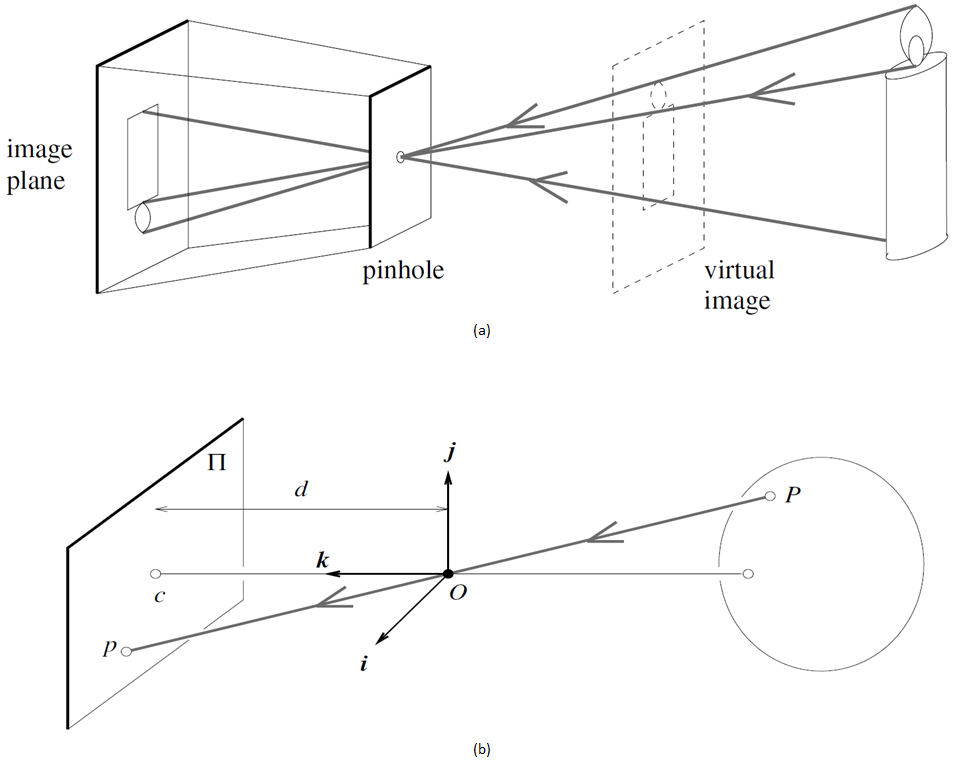
\includegraphics[width=1\textwidth]{camera.png}
	\caption{(a). the pinhole imaging model; (b). geometric model for perspective projection. \cite{Forsyth:2002:CVM:580035}}
	\centering
	\label{figure:camera}
\end{figure}

\subsubsection{Intrinsic and Extrinsic Parameters}
\label{projection}

To project a 3D point in the world coordinate system, first we have to transform this point to the camera coordinate system and then transform it to the image plane. The first transformation depends on the extrinsic parameters while the second rely on intrinsic parameters.

\textbf{Intrinsic parameters} include the focal length $f$ just like the $d$ in Figure \ref{figure:camera} (b), the image coordinates origin $(u_0, v_0)$, and the skewed angle $\theta$ of two image axes. Coordinates in image plane are usually expressed in pixel which can be square or rectangular. So let's assume $\alpha$ and $\beta$ are the value expressed $f$ with horizontal and vertical pixel-meter scales. Therefore, we can finally transform Eq. \ref{eq1} into 
\begin{equation}
\label{eq2}
	\begin{cases}
	u = \alpha \frac{x}{z} - \alpha \cot\theta + u_0, & \\    
	v = \frac{\beta}{\sin\theta} \frac{y}{z} + v_0
	\end{cases}
\end{equation}

When it is written in matrix form as Eq \ref{eq3}, the $3\times3$ matrix $K$ is the intrinsic matrix of the camerac. Note that $P$ is expressed in camera coordinate system and $p$ is in image coordinate system.

\begin{equation}
\label{eq3}
p = K P \Leftrightarrow \frac{1}{z}
\bigl(\begin{smallmatrix}
u\\  v \\1
\end{smallmatrix}\bigr) 
= 
\begin{pmatrix}
\alpha & -\alpha \cot\theta & x_0\\ 0 & \frac{\beta}{\sin\theta}  & y_0\\  0 &0  &1 
\end{pmatrix}
\begin{pmatrix} 
x\\  y\\  z
\end{pmatrix}
\end{equation}

\textbf{Extrinsic parameters} defines a rigid transformation from world coordinate system to camera frame. A rigid transformation has six degree of freedom, including three Euler angles expressed in a $3\time3$ rotation matrix $R$ and three translation components along each axis expressed in a $1\times3$ translation vector $t$. A point expressed in homogeneous coordinates is $P=(x, y, z, 1)^T$. Homogeneous coordinates can simplify various geometric transformations into matrix multiplication \cite{Forsyth:2002:CVM:580035}.  Therefore, this rigid transformation expressed in homogeneous coordinates is 
\begin{equation}
\label{eq4}
P^{C} = T_W^C P^W, where ~~T_W^C = 
\begin{pmatrix}
	R & t\\ 
	0^T& 1
\end{pmatrix}
\end{equation}
$P^{C}$ and $P^W$ are coordinates of the same point expressed in world coordinate system and camera coordinate system respectively. $T_W^C$ is the extrinsic matrix of the camera.

To put it all together, the projection equation in homogeneous coordinates is 
\begin{equation}
\label{eq5}
p = \frac{1}{z} M P^W = \frac{1}{z} K
\begin{pmatrix}
R & t\\ 
0^T& 1
\end{pmatrix} P^W
\end{equation}
where $M$ is the \textbf{perspective projection matrix}.

\section{My Work - Technical Detail}
\begin{figure}[h]		
	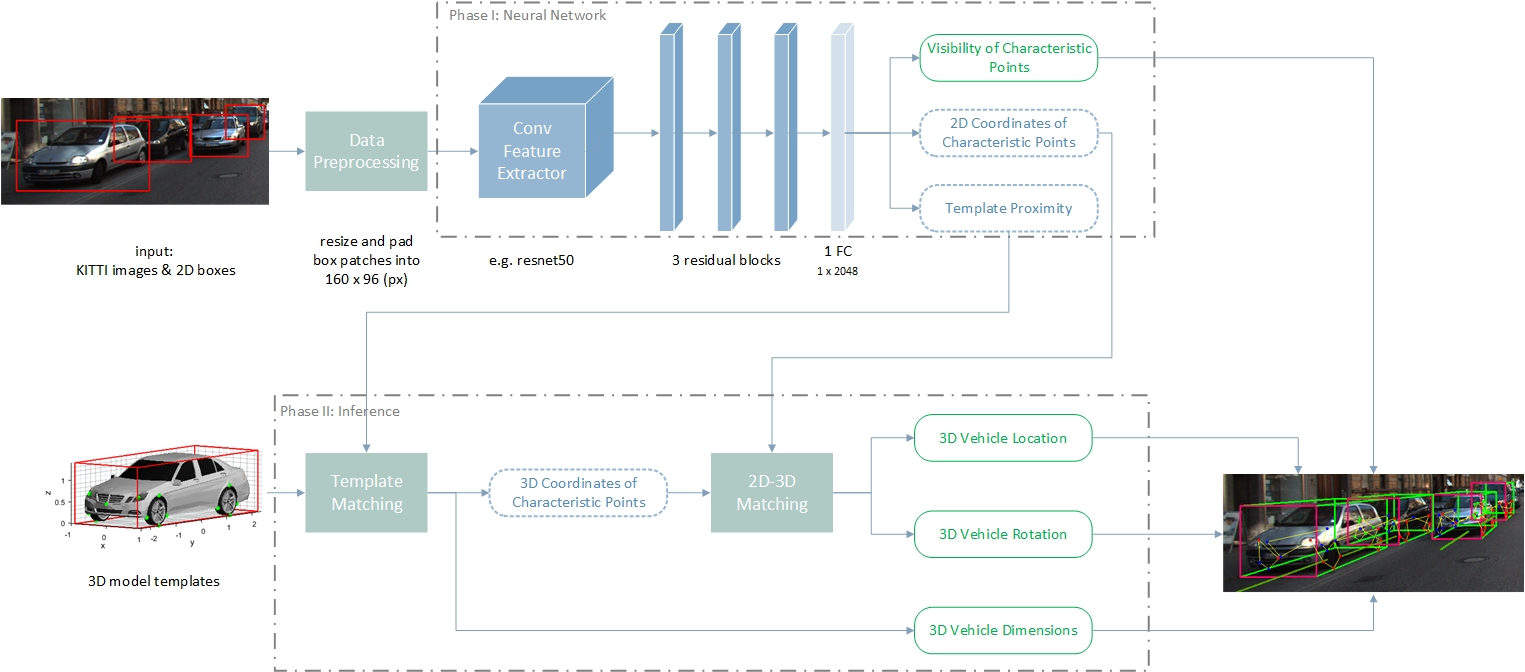
\includegraphics[width=1\textwidth]{app_archi_box_0522.jpg}
	\caption{The Architecture of our Approach}
	\centering
	\label{figure:app_archi}
\end{figure}

In this section, we elaborate our approach for 3D pose estimation of vehicles in monocular images. Our approach is based on 2D vehicle detection, \ie the 2D bounding boxes of vehicles are given as prior, since 2D object detection techniques, such as YOLO \cite{DBLP:journals/corr/RedmonF16}, Faster R-CNN \cite{DBLP:journals/corr/RenHG015}, SSD \cite{DBLP:journals/corr/LiuAESR15}, R-FCN \cite{DBLP:journals/corr/DaiLHS16}, and FPN \cite{DBLP:journals/corr/LinDGHHB16},  have achieve very high accuracy while  end-to-end 3D object detection performance is still primitive.  The overall architecture of the approach is illustrated in Figure \ref{figure:app_archi}. It consists of two main phases. The first one is the CVT Network which takes the KITTI images and the 2D bounding box as inputs and predicts the visibility property and 2D coordinates of all characteristic points, as well as the template proximity. The details are presented in section \ref{network}.  The other phase estimates the 3D location, rotation, and dimension of each vehicle based on the 3D vehicle dataset and the outputs of the CVT Network. Section \ref{inference} demonstrated this phase in detail. The KITTI dataset and the 3D vehicle dataset are described in section \ref{data}.



\subsection{Data and Labelling}
\label{data}
\subsubsection{KITTI Dataset}
The KITTI 2D/3D object detection challenge is dedicated to autonomous driving and releases a dataset containing 7481 images for each one of 4 cameras and their associated labels and calibrations \cite{Geiger2012CVPR}. The dataset covers scenarios of city, residential, road, campus, and person. We only use the images taken by the left colour camera. The example image is shown in Figure \ref{figure:kitti_image}. The associated labels are show in Table \ref{kitti_lable}. The calibration is given as transformation matrix.

\begin{figure}[h]		
	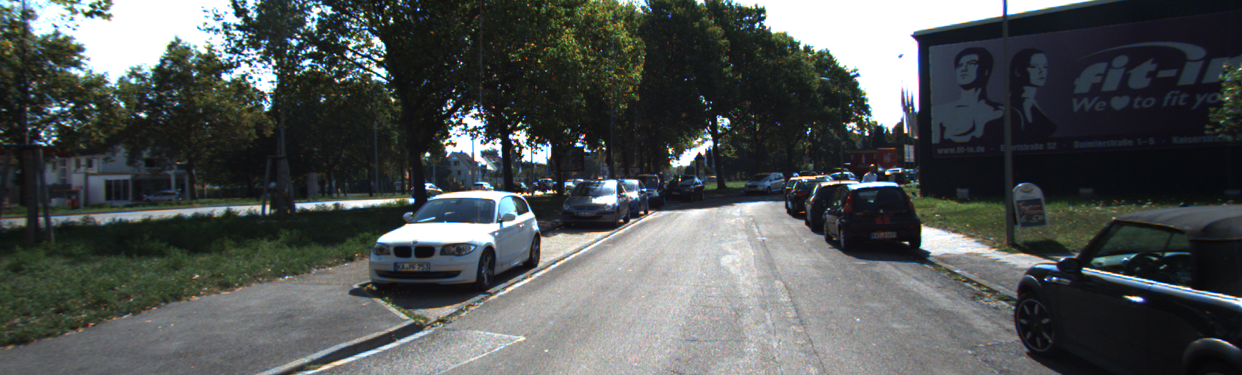
\includegraphics[width=1\textwidth]{000010.png}
	\caption{Example image from KITTI dataset captured by the left colour camera}
	\centering
	\label{figure:kitti_image}
\end{figure}

\renewcommand{\arraystretch}{1.2}
\begin{table}[h]
	\centering
	\caption{Label specification of KITTI dataset}
	\label{kitti_lable}
	\resizebox{\textwidth}{!}{%
		\begin{tabular}{|c|c|l|}
			\hline
			\#Values & Name        & Description                                                                                                                                                             \\ \hline
			1        & type        & \begin{tabular}[c]{@{}l@{}}Type of object: \\ Car, Van, Truck, Cyclist, Tram, Pedestrian, \\ Person\_sitting,  Misc or DontCare \end{tabular}          \\ \hline
			1        & truncated   & \begin{tabular}[c]{@{}l@{}}Float from 0 (non-truncated) to 1,\\ indicating the extent of the object out of the image\end{tabular}                                       \\ \hline
			1        & occluded    & \begin{tabular}[c]{@{}l@{}}Integer indicating occlusion state: \\ 0 = fully visible, 1 = partly occluded, \\ 2 = largely occluded, 3 = unknown\end{tabular}             \\ \hline
			1        & alpha       & Observation angle of object, ranging {[}-pi..pi{]}                                                                                                                      \\ \hline
			4        & bbox        & \begin{tabular}[c]{@{}l@{}}2D bounding box of object in the image (0-based index): \\ contains left, top, right, bottom pixel coordinates ($x_1$, $y_1$, $x_2$, $y_2$)\end{tabular} \\ \hline
			3        & dimensions  & 3D object dimensions: height, width, length (in meters)                                                                                                                 \\ \hline
			3        & location    & 3D object location x,y,z in camera coordinates (in meters)                                                                                                              \\ \hline
			1        & rotation\_y & Rotation ry around Y-axis in camera coordinates {[}-pi..pi{]}                                                                                                           \\ \hline
		\end{tabular}%
	}
\end{table}

\subsubsection{3D Vehicle Dataset}
\label{cad_models}
This dataset is intended to encode the diversity of vehicles by means of type, dimension, and chassis shape. It is created based on a selected subset of synthetic 3D CAD models\cite{NIPS2012_4562}. We only include the well-aligned and  symmetrical models, and also take the dimension and type into consideration. We classify all the models into six categories: Mini, Hatchback, Sedan, SUV, Wagon, and Van. And for each category,  subcategories are marked out according to their dimensions and shapes in order to make a refined selection.  The statistic of dimensions is well distributed and each existing car can be classified into one category exclusively.

\begin{figure}[h]		
	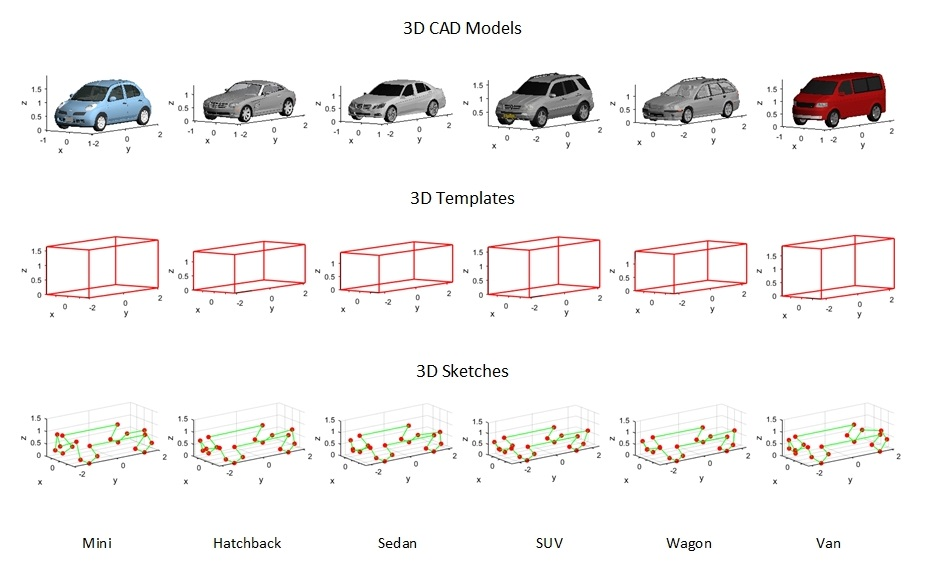
\includegraphics[width=1\textwidth]{vehicle_dataset.jpg}
	\caption{Six vehicle categories of the 3D vehicle dataset. Each vehicle model is associated to a 3D CAD model, a 3D template, and a 3D sketch.}
	\centering
	\label{figure:vehicle_dataset}
\end{figure}

Our final dataset consists of 54 valid vehicle models. Each vehicle model has a 3D CAD model, a 3D template, and a 3D sketch correspondingly, as shown in Figure \ref{figure:vehicle_dataset}. All these three representation are aligned in canonical view and share an identical object coordinate system. The CAD models are created based on real vehicles and have all the geometry information with them. The 3D templates represent the vehicles' dimensions. The 3D template associated to the 3D model $k$ is denoted as $t_k = (h_k, w_k, l_k)$ where $h_k, w_k$ and $l_k$ represent the height, width, and length of the model respectively. 

The  3D sketches indicate the chassis shapes. Each 3D sketch consists of 20 characteristic points around the chassis with each point denoting one part of the vehicle. So the $k^{th}$ sketch is denoted as $S_k^{3d}  = (p_1, p_2, ... p_{20})$, where $~p_i = (x_i, y_i, z_i)$. The reason why we choose the points around chassis as feature points is that their geometric relationship is more stable than points in other places. Because the chassis part is more about functionality than appearance attraction compared to other parts of the vehicle,  \eg the upper part. In this way, the sketches can be more universal so that they can represent a wider range of vehicles, which reduces the number of models required and further increases the computational efficiency. 

In order to create the 3D sketches, we implement a labelling tool, shown in Figure \ref{figure:label_cad}. It is capable to label the 3D coordinates for all the characteristic points associated to each vehicle.[\tbd  should it be elaborated in detail]

\begin{figure}[h]		
	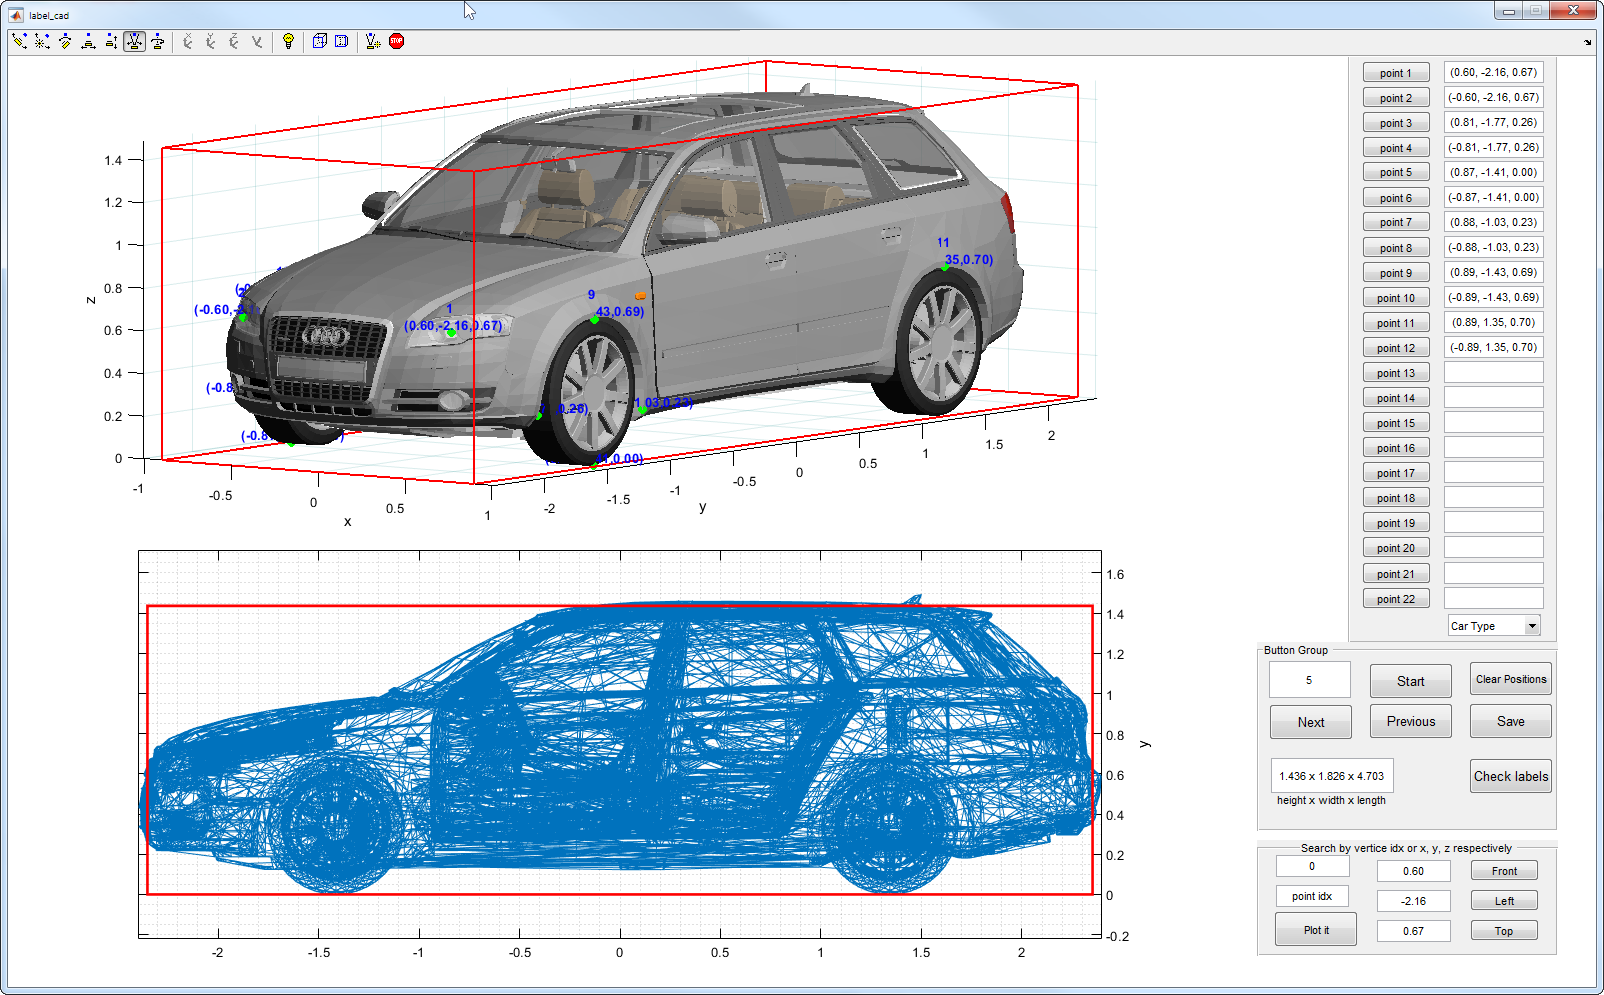
\includegraphics[width=1\textwidth]{label_cad.png}
	\caption{Labelling tool for 3D sketches}
	\centering
	\label{figure:label_cad}
\end{figure}

\subsubsection{Labelling for KITTI Dataset}

Our approach requires three extra kinds of labels to training the CVT Network, \ie 2D coordinates and visibility property of characteristic points and template proximity, as shown in Table \ref{new_label}.  Labelling is never a trivial task. Due to the demanding workload of manual labelling and the cases where it is almost impossible to label the small vehicles in image manually, we propose an automatic label generation method. It is able to make use of the 3D vehicle dataset and the KITTI dataset to generate these three additional kinds of ground truth.

\renewcommand{\arraystretch}{1.2}
\begin{table}[h]
	\centering
	\caption{Specification of three additional labels}
	\label{new_label}
	\resizebox{\textwidth}{!}{%
		\begin{tabular}{|c|c|l|}
			\hline
			\#Values & Name        & Description                                                                                                                                                             \\ \hline
			2x20        & 2D coordinate  & $(x, y)$, location of 20 characteristic points in image coordinates                                                                                                                \\ \hline
			1x20        & visibility    & \begin{tabular}[c]{@{}l@{}}Integer indicating visibility property of each point: \\ 0 = visible, 1 = occluded, \\ 2 = self-occluded, 3 = truncated\end{tabular}    \\ \hline
			3x54        & template proximity & \begin{tabular}[c]{@{}l@{}} A vector $\mathit{T_{i}}$ represents the dimension ratios \\ between each model and the vehicle  \end{tabular}   \\ \hline
		\end{tabular}%
	}
\end{table}


\paragraph{2D Coordinates}

2D coordinates of key points of each vehicle in image coordinates is generated by projecting the 3D sketch of this vehicle to the image. The vehicle's 3D sketch is selected via template-matching, \ie the best-matching sketch is the one whose associated template is closest to the vehicle's dimensions. The 3D-2D projection is performed based on the given intrinsic and extrinsic parameters, as shown in Figure \ref{3D_2D_projection}. The intrinsic parameters are given as calibration by KITTI and the extrinsic parameters are given as 3D object dimensions and rotation ry in KITTI labels. KITTI makes a simplified assumption here that the vehicle only rotates around the yaw axis but not roll or pitch axis. One example of the labelled 2D coordinates is shown in Figure \ref{visibilie_eg}.

\begin{figure}[h]		
	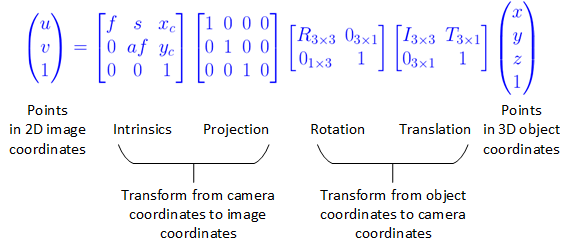
\includegraphics[width=1\textwidth]{projection_matrix.png}
	\caption{3D-2D projection}
	\centering
	\label{3D_2D_projection}
\end{figure}

\begin{figure}[h]		
	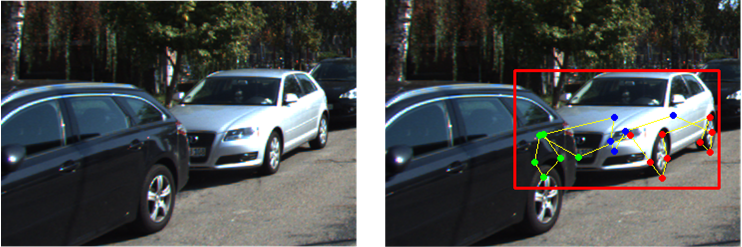
\includegraphics[width=1\textwidth]{visibilie_eg.png}
	\caption{Example of 2D coordinates and visibility of one vehicle. The left image is one patch of KITTI image. The left image is the one after labelling. The points indicate the 2D coordinates and the color indicates the types of visibility: red for visible, green for occluded, and blue for self-occluded.}
	\centering
	\label{visibilie_eg}
\end{figure}



\paragraph{Visibility}
\label{visibility}

As an example of the labelled visibility shows in Figure \ref{visibilie_eg}, the visibility property of characteristic points is classified into four scenarios: 

\begin{enumerate}[\hspace{0.4cm} i.]
	\itemsep-0.5em 
	\item Visible if the point can be seen directly;
	\item Occluded if the point is occluded by other objects;
	\item Self-occluded if the point is blocked out by the vehicle itself;
	\item Truncated if the point exceeds the boundaries of the image. 
\end{enumerate}

\begin{figure}[h]		
	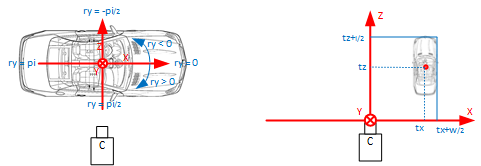
\includegraphics[width=1\textwidth]{visibility_imp.png}
	\caption{Visibility labelling mechanism. The left image shows the rotation ry in the camera coordinate system, which helps distinguish visible or self-occluded case. The left image shows the location of the vehicle in the camera coordinate system, which helps defined the occluded situation.}
	\centering
	\label{visibility_imp}
\end{figure}

The visibility of each point is determined by its position, \ie the 2D coordinate in image.  Being visible or self-occluded is distinguished by means of rotation ry of each vehicle. As the right plan sketch in Figure \ref{visibility_imp} shows, the rotation ry can indicate unambiguously which faces of the vehicle are facing to or away from the camera. If the points are on the observable faces, they  are labelled as visible,  otherwise they are classified as self-occluded. Occluded case happens when the 2D coordinate of the point falls into the 2D bounding box of a former object. The object is defined as former when it locates in the region enclosed by the axes and two solid blue line in the left schematic plot of Figure \ref{visibility_imp} if the vehicle is on the first quartile.  And when the vehicle is on the second quartile, it's just a mirrored case. Truncated is defined that its 2D coordinate exceeds the boundaries of the image. The size of KITTI images are determined which makes it easy to implement. The truncated property has the highest priority, the occluded underlies , the self-occluded or the visible is considered at last.


\paragraph{Template Proximity}
\label{template}

Template proximity of one vehicle is encoded as a vector $\mathit{T_{i}}$ which is defined as $\mathit{T}_i = \{r_k\}_{k \in \{1,.., K\}}$, where $\mathit{K}$ denotes the number of 3D vehicle models and  $r_k~=~(r_h,r_w,r_l)$ corresponds to three scaling ratios between the dimensions (\ie height, width, and length) of each model and the vehicle's respectively. The vector $\mathit{T_{i}}$ represents the similarity between each model and the vehicle. The most similar model is the one whose $r_k$ is closest to $(1, 1, 1)$.

\subsubsection{Notations}
In sum, based on the KITTI image and 3D vehicle models, each vehicle can be defined by seven critical attributes:
\[  \{D, B^{2d}, ~B^{3d}, ~C^{2d}, ~C^{3d}, ~V, ~T\}  \]
$D = (h, w, l)$ represents the dimensions of the vehicle. $B^{2d} = (c_u, c_v, w, h)$ defines the 2D bounding box in image with $(c_u, c_v)$ denoting its center,  $w$ for its width and $h$ for its height. $B^{3d} = (o, \theta, d)$ where $o = (c_x, c_y, c_z)$ is the center, $\theta$ is the rotation ry around the yaw axis, and $d = (w, h, l)$ is its dimensions. $C^{2d}  = \{(u_i, v_i)\}_{i \in \{1, ...,20\}}$ represents the 2D part coordinates in image plane, while $C^{3d}  = \{(x_i, y_i, z_i)\}_{i \in \{1, ...,20\}}$ denotes the 3D part coordinates in world coordinate system. $V = \{v_i\}_{i \in \{1, ...,20\}}$ is the visibility for all the characteristic points in the vehicle.  $T = \{{(r_{h},r_{w},r_{l})}_k\}_{k \in \{1, ...,54\}}$ is the template proximity vector.

\subsection{Deep CVT Network}
\label{network}
This subsection describes the details of the Deep CVT Network, including its architecture, implementation, and training.

\begin{figure}[h]		
	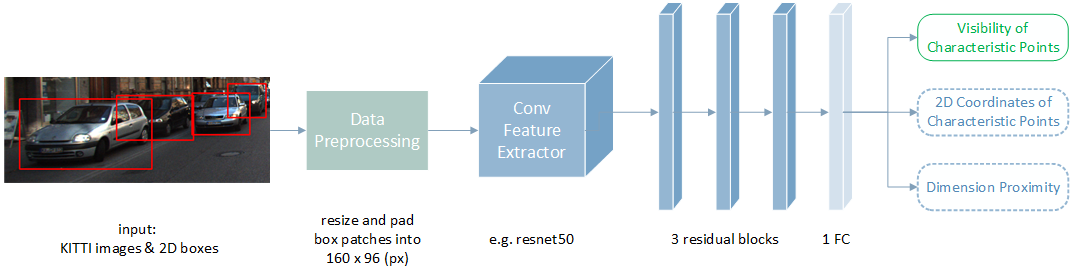
\includegraphics[width=1\textwidth]{NN_archi_box_0522.png}
	\caption{The Architecture of Deep CVT Network}
	\centering
	\label{figure:nn_archi}
\end{figure}

\subsubsection{Architecture}
The neural network is to learn a map from an N-dimensional  input space to an M-dimension output space. The map consists of several stages, called layers of the network, written as
\begin{equation}
Y = l_L(...l_2(l_1(X))), where ~Y \in {\mathbb{R}^M}, ~X \in {\mathbb{R}^N}
\end{equation}

Even through there are various layers, most layers  is composed of neurons, the basic computation element and most neurons are realized by linear and non-linear operations as 
\begin{equation}
a_{ij} = \sigma(W_{ij}^T X_i +b_j)
\end{equation}

where $a_{ij}$ is the result of the $i_th$ neuron in the $j_th$ layer, $\sigma$ is the activation function and $W_ij$ and $b_j$ are the weights vector and bias applied to input vector $X_i$.  The pooling layer is a special case which performs downsampling operations, such as max pooling \cite{Boureau:2010} and average pooling \cite{6460871}.

As shown in Figure \ref{figure:nn_archi}, our network follows the standard CNN architecture established in LeNet-5 \cite{726791}. It stacks a set of convolutional layers and pooling layers as a feature extractor, \tbd followed by 3 residual blocks and one fully-connected layers to refine the features, and three kinds of output layers in the end. The goal of this network is to learn the 2D coordinates and visibility property of 20 interest points and the template proximity of the vehicle, given the RGB images captured by a monocular camera.

\paragraph{Input Layer}
The input layer accepts the input RGB images and feeds them into the network. In theory, images with arbitrary size can be accepted, but to make it more efficient, we use images with fixed resolution (96 x 160).  In this way, multiple images can be processed in one batch in order to reduce the variance of parameter updates and make the best use of highly optimized matrix optimizations during training \cite{DBLP:journals/corr/Ruder16}.

Since our approach is based on 2D object detection, each image contains at least one whole vehicle . To obtain these images, we first crop the patches defined by the 2D bounding box, then resize them to match one predefined dimension (96 or 160), and finally put the resized images in the center of the 96 x 160 canvas and padded with zeros for other pixel positions. We choose 96 x 160 as the fixed size because they are the means of sizes of all original patches so that we don't have to rescale the patch too much.  Some examples are shown in Figure \ref{figure:patches}.

\begin{figure}[h]		
	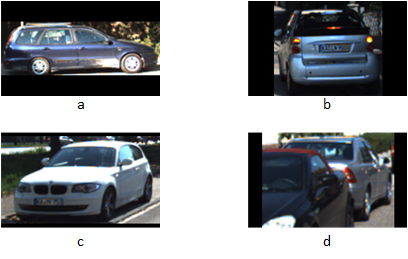
\includegraphics{patches.png}
	\caption{Examples of input images: a. the side view, b. the back view, c. the front view, d. the occluded case}
	\centering
	\label{figure:patches}
\end{figure}

\paragraph{Hidden Layers}
The hidden layers in out network consist of a feature extractor, 3 residual blocks \cite{DBLP:journals/corr/HeZRS15}, and a fully-connected layer. Both the feature extractor and residual blocks are composed of convolutional layers and pooling layers.

The feature extractor is actually one of available neural network models built in the Keras library \cite{chollet2015keras}, \ie VGG16, VGG19, Xception, ResNet50, \etc It is trained to  learn deep distributed hierarchical nonlinear representations of the input images.

 ResNet50 \cite{DBLP:journals/corr/HeZRS15} is chosen to be the benchmark model because it can ease the training and accelerate the convergence, especially for the fine tuning. It is well known that there are two main obstacles that hamper the training of deep neural networks: the vanishing/exploding gradient problem \cite{Bengio:1994:LLD:2325857.2328340, pmlr-v9-glorot10a} and the degradation problem that as the network is built deeper, the accuracy gets saturated or even degrades sharply \cite{DBLP:journals/corr/He014}. Residual nets are designed to address these two problems. Instead of learning the direct mapping from input to output, it learns a residual mapping first and then add the input to it, which just as Figure \ref{figure:residual_blocks} (a) shows. The paper validates that it is easier to learn the residual mapping than the direct one and the gradient can always pass through along the shortcut connections. Figure \ref{figure:residual_blocks} (b) and (c) shows two building blocks in our network. (b) is an identity block where the dimensions of input and output matches, while (c) is a linear projection block where the right branch performs $1\times1$ convolution to match the dimensions because the final addition is performed element-wisely.

\begin{figure}[h]		
	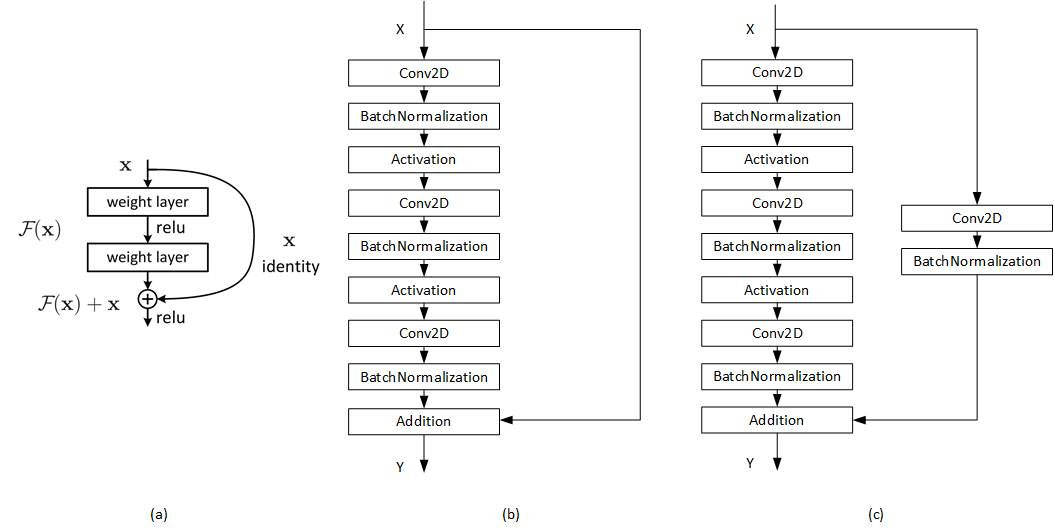
\includegraphics[width=1\textwidth]{residual_blocks.png}
	\caption{(a). a residual block \cite{DBLP:journals/corr/HeZRS15}, (b). an identity residual block in our network, (c). a linear projection residual block in our network}
	\centering
	\label{figure:residual_blocks}
\end{figure}

The last three residual blocks and a fully-connected layer is designed to learn non-linear combinations of the extracted features and then forward them to the output layers.

For all hidden layers, we all apply ReLU as the activation function. The function is

\begin{equation}
\label{relu}
f(z) = \max \{0, z\} ~~~~where~ z = W^TX+b
\end{equation}
This is a piecewise linear function consisting of two linear pieces, which makes the gradients through a rectified linear unit stay large and consistent whenever the unit is active. Papers \cite{pmlr-v15-glorot11a, Nair:2010:RLU:3104322.3104425, DBLP:journals/corr/JarrettKGL16} have validated that networks activated by ReLU can achieve much better performance than others. ReLU preserves many properties that make the model easy to optimize with gradient-based methods and generalize well, while introducing non-linearity into the model \cite{Goodfellow-et-al-2016}. 

\paragraph{Output Layers}
\label{output}

Our network has three kinds of output layer for the three tasks respectively. For 2D coordinates regression, a 40-neuron layer with linear activation function is provided.  Each neuron's output indicates one coordinate value, \ie $x_i$ or $y_i$.  20 coordinates are arranged in an ascending order. For visibility characterization, we implement 20 independent quaternary classifiers for 20 points. Each classifier is associated with a softmax activation function \cite{Bishop:2006:PRM:1162264} which outputs four values representing the probabilities of each target class over all possible classes. Template proximity is equipped with a 154-neuron linear layer for regression.  Each neuron indicates one ratio element of the template proximity vector. Eq.\ref{linear} is a linear activation function while Eq.\ref{softmax} is a softmax activation function.

\begin{equation}
\label{linear}
out_i = W_i^TX_i+b_i
\end{equation}

\begin{equation}
\label{softmax}
out_i = \frac{e^{W_i^TX_i+b_i}}{\sum_{k=1}^K e^{W_k^TX_k+b_k}}
\end{equation}


\subsubsection{Training}

\paragraph{Multi-task Learning}
As mentioned in Section \ref{output}, our network has totally 22 output layers. This implementation makes use of multi-task learning (MTL) where multiple learning tasks are trained parallel based on the shared features. Caruana has validated that tasks trained in MTL have better generalization performance than trained in a single-task learning mode \cite{Caruana1997}. And he summarizes that this improvement results from leveraging the domain-specific information contained in the training signals of other related tasks \cite{Caruana1997}. Therefore, we follow this paradigm to design our network in order to achieve better performance.

\paragraph{Loss Functions}
\label{loss_functions}
The learning of 2D coordinates and template proximity are regression tasks so that a robust smooth $L_1$ loss function \cite{DBLP:journals/corr/Girshick15} is chosen for them. We modify it as

\begin{equation}
\label{eq10}
smooth_{L_1}(x) =
\begin{cases}
~x^2 ~~~~~~~~~~~~if ~\left | x \right |< 0.25 & \\    
~\left | x \right | - 0.1875 ~~~~~otherwise   
\end{cases} 
where  ~ x=\widehat{y} - y
\end{equation}
Compared to $L_2$ loss, it is less sensitive to outliers and no special attention is required to pay in order to prevent gradient exploding problem\cite{DBLP:journals/corr/Girshick15}. Besides, when applied with gradient-based optimization, $L_1$ loss and $L_2$ loss often result in poor performance \cite{Goodfellow-et-al-2016}.

For visibility characterization, we develop a model for probabilistic classification so that categorical cross-entropy is used as the loss function. It is also known as the negative log-likelihood \cite{Goodfellow-et-al-2016}, defined as:

\begin{equation}
\label{eq11}
L_{cce} =\frac{1}{N} \sum_{n=1}^N H(y,\widehat{y}) = -\frac{1}{N}\sum_{n=1}^N \sum_{i=1}^c y_{n,i} \log \widehat{y}_{n,i}
\end{equation}

where $H(y, \widehat{y})$ denotes the cross-entropy between the ground truth probability distribution $y$ and the predicted $\widehat{y}$, and $y_{n,i} $ represents the true probability of $i_{th}$ class for the $n_{th}$ data example $\widehat{y}_{n,i}$ is the estimated. It is a continuous convex loss function which measures the discrepancy between the true and estimated distributions multi-class classification tasks \cite{DBLP:journals/corr/abs-1802-09941} which means it can measure the degree of correctness, \ie it can distinguish between "nearly correct" and "totally wrong" cases.  Therefore, it outperforms other loss functions in classification tasks and then becomes ubiquitous in deep learning nowadays.

Therefore training objective is expressed as the total loss of all tasks, written as:
\begin{equation}
\label{eq12}
L_{total} = \lambda_{coord} L_{coord} + \lambda_{temp} L_{temp} + \lambda_{visib}\sum_{i=1}^{20} L_{visib~i}
\end{equation}

where $\lambda_{coord}, \lambda_{temp}$, and $\lambda_{visib}$ are loss weights for these three kinds of tasks respectively. Loss with higher weights has more impact on the gradients and thus tunes the parameters perform better for its corresponding task.

\paragraph{Normalization}
\label{normalization}
Normalization is an important pre-processing step in deep learning which ensures that each feature has a similar data distribution. This is usually done by restricting the features in certain range or standardizing their ranges. It can enhance the learning capability of the network and speed up the convergence substantially  because it can reduce the bias among features and decrease the low and high frequency noisy in data \cite{Jayalakshmi2011}. The speed-up mechanism can be concluded from Figure \ref{figure:contour}. If we initialize the network at point A in Figure \ref{figure:contour} (a), the gradient-descent update routine will oscillate along the long axis of the eclipse, which definitely takes more time to reach the optimum than any arbitrary initial point in Figure \ref{figure:contour} (b) where the update trajectory is almost a straight line for any starting point  to the minimum. Besides, this also helps the performance because the update trajectory oscillates less around the minimum for case (b) than case (a) so that it is more possible for case (b) to reach the optimum.

\begin{figure}[h]		
	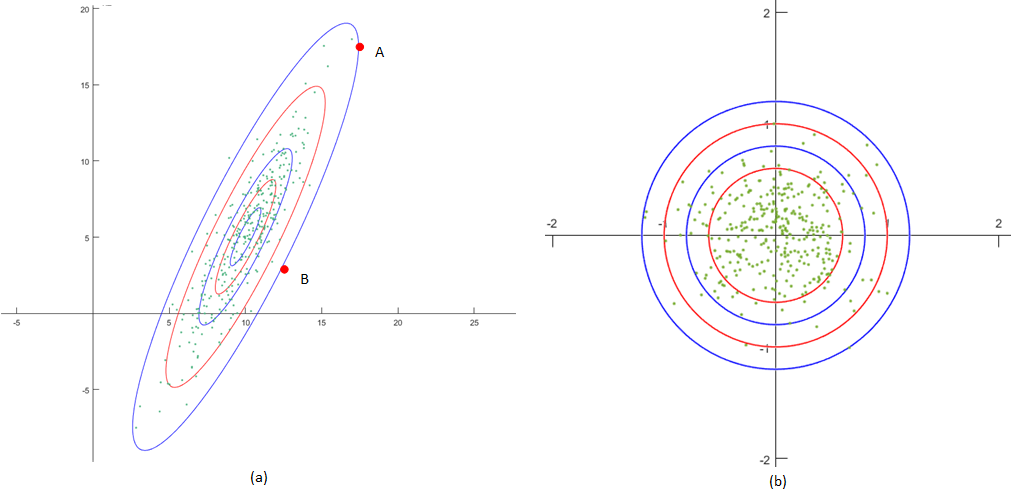
\includegraphics[width=1\textwidth]{contour.png}
	\caption{(a). data distribution before normalization, (b). data distribution after normalization}
	\centering
	\label{figure:contour}
\end{figure}

Our network takes RGB images as input so that pixel intensity is the input feature. The technique we use to normalize the image is channel mean subtraction, used in \cite{DBLP:journals/corr/SimonyanZ14a, DBLP:journals/corr/GirshickDDM13}, which centers all the features around the origin along each dimension.As mentioned in CS231N \cite{CS231N}, mean channel subtraction is enough for CNNs and the original range of pixel values is determined, \ie $[0, 255]$.

The range of ground truth influences the loss. In order to make the three labels impact similarly on the loss, we normalize them. For visibility, we use one-hot-encoding \cite{One-hot} to encode its classes so that it only has value 0 or 1. The value of 2D coordinates $C^{2d}  = \{p_1, p_2, ...,p_{20}\}$varies a lot so that we normalize them w.r.t. the associated 2D bounding box $B^{2d} = (c_u, c_v, w, h)$ \cite{DBLP:journals/corr/ChabotCRTC17}. The normalized 2D coordinates $\overline{C}^{2d}  = \{\overline{p}_1, \overline{p}_2, ...,\overline{p}_{20}\}$ ranges $[-1, 1]$, where
\begin{equation}
\overline{p}_i  = (\frac{u_i - c_u}{w}, \frac{v_i - c_v}{h})
\end{equation}

The template proximity vector $T$  is normalized with $\log$ function element-wisely \cite{DBLP:journals/corr/ChabotCRTC17}, resulting in $\overline T$ so that the range falls into $[-1, 1]$, too.

Moreover, as Sergey \etal \cite{DBLP:journals/corr/IoffeS15}states the variation of each layer's input distribution during the training makes the training complicated and hard to converge quickly so that we apply Batch Normalization (BN) to alleviate the internal covariate shift phenomenon.  BN normalizes the summed activations of each layer to a distribution of zero mean and unit variance. The mean and variance of each activation is computed on each mini-batch. By doing so, much larger learning rate can be used for training and no special attention has to pay on parameter initialization. 
 
\paragraph{Regularization}
Regularization techniques are used to address the overfitting problem in order to make an algorithm not only perform well on the training data but also on the test data, the previously unseen data \cite{Goodfellow-et-al-2016}. Overfitting results from either that the algorithm is too complicated for the data or that the sampled data is not able to represent the internal pattern. Normally, we design an algorithm to model  the data pattern exhaustively first and then apply regularization techniques to make the algorithm generalize well.  

In the data aspect, we use data augmentation as a regularization. The best way to address overfitting is to train the model on more data, while the amount of data is restricted for one dataset. Therefore we generate some synthetic data. Since our network involves with classification and regression tasks, we mainly enlarge the dataset via horizontal and vertical flipping and scaling. 

In the architecture aspect, Batch Normalization \cite{DBLP:journals/corr/IoffeS15} is used as the regularization in each layer. BN enables the network to obtain the information of the training sample and the others in mini-batch simultaneously so that it does not generate deterministic dependency on this training sample. Therefore BN can replace Dropout \cite{JMLR:v15:srivastava14a} to be the regularization for our convolutional network. 

Besides, Multitask Learning is another technique we used to improve generalization performance. 
In our network, the learning representation is shared across all tasks so that the parameters shared are constrained to bias towards one specific task, \ie only the representation that is useful for more than one can be kept \cite{Goodfellow-et-al-2016}.  Therefore statistical strength of the parameters is highly enhanced \cite{Baxter:1995:LIR:225298.225336}.

During the training, early stopping is applied to prevent the model being trained too complex to fit the test data. As Figure \ref{figure:early_stopping} shows, we halt the training when the validation error stops decreasing.  The stopping point is when the learned model can represent the pattern of validation data most. It regards the number of training epochs as a hyperparameter and can effectively tune it to be optimal \cite{DBLP:journals/corr/abs-1206-5533},  because early stopping can restrict the global learning capacity of a large network to fit simpler dataset without affecting the backpropagation to control the learning capacity locally \cite{Caruana:2000:ONN:3008751.3008807}.


\begin{figure}[h]		
	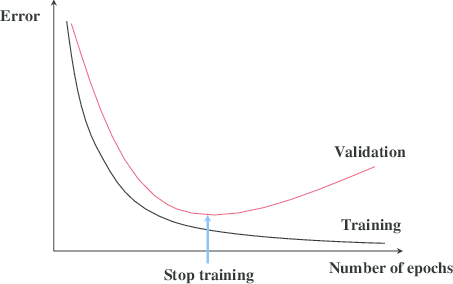
\includegraphics{early_stopping.png}
	\caption{Early stopping}
	\centering
	\label{figure:early_stopping}
\end{figure}

\paragraph{Parameter Initialization}

Transfer learning is proposed to transfer the representation learned from one task to another related task \cite{Pan:2010:STL:1850483.1850545}. As is known that CNNs learn more abstract features in a deeper layer. It is not surprising to find that, for visual tasks, shallow layers learn low-level features, \eg edges, corners, changes in lighting, \etc, which are shared across datasets and tasks. Moreover, Yosinski \etal validate \cite{DBLP:journals/corr/YosinskiCBL14} that initializing a network with transferred features can improve the generalization capability hugely and Yoshua \etal \cite{NIPS2006_3048} confirm that this initialization put the start point closer to a local minimum than random initializations, resulting in accelerating convergence.

Therefore we initialize our feature extractor with parameters learned on ImageNet dataset \cite{DBLP:Russakovsky14} and the three residual blocks with parameters trained on the KITTI dataset. The fully-connected layer is initialized from a zero-mean Gaussian distribution with standard deviation 0.01 and all the output layers are initialized with zeros.


\paragraph{Learning Algorithms / Optimization}

Optimization is a task of finding the value $x$ in order to minimize or maximize some objective function $f(x)$. One most powerful optimization technique category in deep learning is gradient-based.

As is known, the derivative $f'(x)=\frac{\text{d}y}{\text{d}x}$ specifies how to make a small change $\epsilon$ of the input $x$ to get the corresponding change in the function:
\begin{equation}
	f(x + \epsilon)~ \approx ~ f(x) + \epsilon f'(x).
\end{equation}

Thus, the derivative tells the direction to minimize a function, i.e. it can point out how to change $x$ to make a small update. One popular algorithm, gradient descent \cite{gd1847}, makes use of the derivatives and update the input $x$ directly as:

\begin{equation}
x = x - \alpha {\triangledown} _x f(x)
\end{equation}

where $\alpha$ is the learning rate, a positive real value to decide the size of an update step. The examples in Figure \ref{figure:optimization} (a) show how the update works.  A deep network often consists of many layers so that back-propagation algorithm \cite{Rumelhart:1988:LRB:65669.104451} is used to compute the gradient for each parameter in different layers of the objective function based on the chain rule of calculus.

\begin{figure}[h]		
	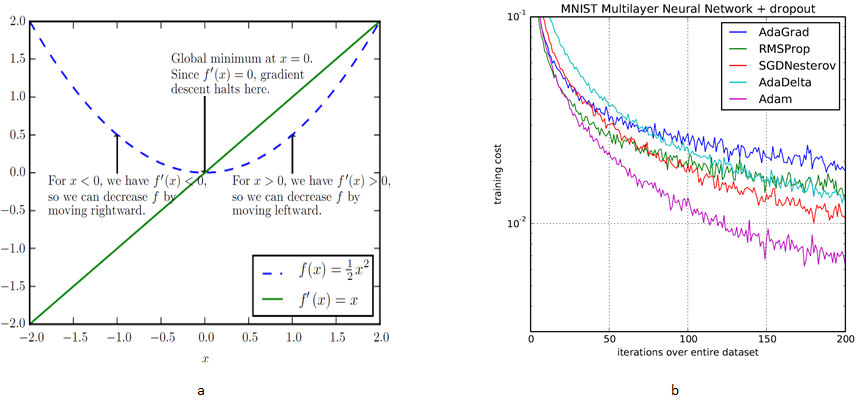
\includegraphics[width=1\textwidth]{optimization.png}
	\caption{(a). examples to show how gradient decent makes use of derivatives to reach a minimum \cite{Goodfellow-et-al-2016}, (b). performance of optimization algorithms in the same setting \cite{DBLP:journals/corr/KingmaB14}}
	\centering
	\label{figure:optimization}
\end{figure}

In deep learning, the input to the objective function is often multidimensional so that it probably has many local minima and saddle points, which renders huge difficulties to optimization. Therefore we usually take in a compromise scenario where the value $x$ makes $f$ really low but not necessarily globally minimal \cite{Goodfellow-et-al-2016}.

The optimization algorithm we used is Adam \cite{DBLP:journals/corr/KingmaB14} which is robust and efficient in memory and computation for the optimization of stochastic objectives with high-dimensional parameters spaces. It makes use of both the gradient and its momentum to update parameters as: 

\begin{algorithm}[H]	
	\While{$x_t$ not converged}{
		$ t = t + 1 $\;
		$ g_t = {\triangledown} _x f(x_{t-1}) $\;
		$ m_t = \beta_1 m_{t-1} + (1-\beta _1) g_t$ \;
		$ v_t = \beta_2 v_{t-1} + (1-\beta_2) g_t^2 $\;
		$ \hat{m}_t = \frac{m_t}{1 - \beta _1^t} $\;
		$ \hat{v}_t = \frac{v_t}{1 - \beta_2^t}  $\;
		$ x_t = x_{t-1} - \alpha \frac{\hat{m}_t}{\sqrt{\hat{v}_t} + \epsilon}$\;
	}
	%\caption{Adam algorithm update mechanism}
\end{algorithm}

where $ t $ denotes the current iteration, $\alpha$ is the learning rate, $\beta_1$ and $\beta_2$ are two exponential decay rates, and $\epsilon$ is a small scalar to prevent zero-division.

From the Figure \ref{figure:optimization} (b), we can see that Adam can make the learning task converge relatively faster and has lower training error so that we follow this guide to apply Adam in our optimization of CVT Network.

\subsection{Inference}
\label{inference}

As shown in Figure \ref{figure:inference}, he inference phase consists of two main steps: template matching to obtain the 3D coordinates of characteristic points and 3D dimensions for the objective vehicle and 2D-3D matching to recover the 3D vehicle location and rotation.

\begin{figure}[h]		
	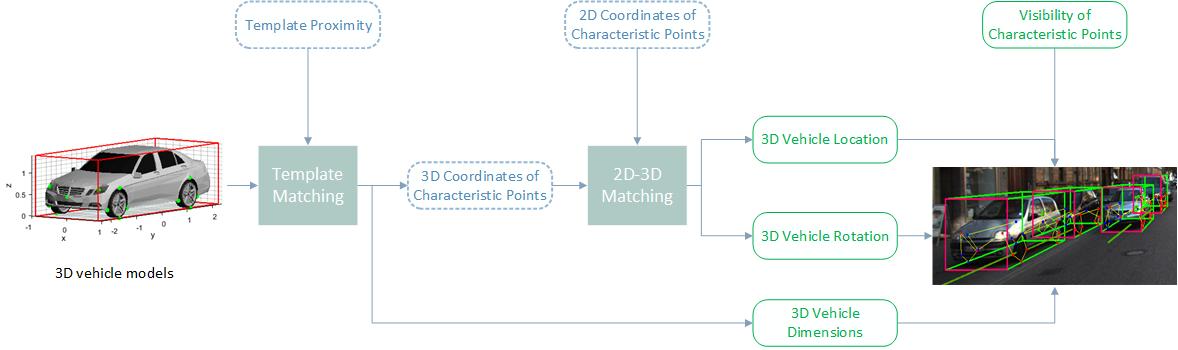
\includegraphics[width=1\textwidth]{inference_0522.png}
	\caption{The Architecture of our Approach}
	\centering
	\label{figure:inference}
\end{figure}

\subsubsection{Template Matching}

Template matching is based on the 3D template dataset and the learned template proximity for the objective vehicle in image. As defined in section \ref{template}, template proximity vector, ${T} = \{{(r_h,r_w,r_l)}_k\}_{k \in \{1,.., K\}}$, measures the dimension similarity between the target vehicle and 3D vehicle models. The best matching model is the one whose dimensions $(h, w, l)$ has the least distance to the target vehicle's dimension $(\bar{h}, \bar{w}, \bar{l})$, \ie the corresponding scaling ratios, $(r_h,r_w,r_l)$, is closest to $(1, 1, 1)$. 

Let's denote the best matching template for the target vehicle $m$ as $t_j$ and the dimension ratio between the target vehicle and the best matching model as $r_j = (r_h,r_w,r_l)$. Then its corresponding 3D sketch is $S_j^{3d}  = (p_1, p_2, ... p_{20})$. To get the target vehicle's dimension $D_m$, we apply the scaling ratios, $(r_h,r_w,r_l)$, to $t_i$ as
\begin{equation}
	D_m = t_j \cdot r_j =  (h_j, w_j, l_j) \cdot (r_h,r_w,r_l) = (h^m, w^m, l^m)
\end{equation}

In the same way, we can get the 3D coordinates of the interest points of the objective vehicle,$C_m^{3d}$, as
\begin{align}
C_m^{3d} &= S_j^{3d} \cdot r_j \nonumber \\  
					  &=  {\{(x_i, y_i, z_i)\}}_{i \in \{1, ...,20\}} \cdot (r_h,r_w,r_l) \nonumber \\  
					  &= {\{(x_i^m, y_i^m, z_i^m)\}}_{i \in \{1, ...,20\}} \qquad {} 
\end{align}

\subsubsection{2D-3D Matching}

Based on the projection mechanism described in section \ref{projection}, the 2D coordinate of one point in image coordinate system can be generated via projecting the 3D point in the world coordinate system with the perspective projection matrix to the image plane. This process is described in Figure \ref{3D_2D_projection}. Now the CVT network predicts the 2D coordinates,$C_m^{2d}$ of the 20 interest points of the target vehicle $m$ and the template matching process provides the corresponding 3D coordinates, $C_m^{3d}$. Then the 3D-2D projection equation in homogeneous coordinates becomes:
\begin{equation}
	C_m^{2d} =   K_{3\times 4}
	\begin{pmatrix}
	R_{3\times 3} & t_{3\times 1}\\ 
	0_{1\times 3}& 1
	\end{pmatrix} C_m^{3d}
\end{equation}

\tbd [add the optimization equation for 2D-3D matching here]
where $K_{3\times 4}$ is the given camera calibration matrix, $R_{3\times 3}$ and $t_{3\times 1}$ are the rotation and translation to be computed. It is easy to compute the rotation and translation of the target vehicle in the camera coordinate system with the standard 2D-3D matching algorithm, EPnP \cite{Lepetit2008}. The KITTI data simplifies the rotation to one dimension, $r_y$, so that we follow this convention. Translation is the 3D coordinate of the origin of the vehicle so that it can represent the location of the vehicle in camera coordinate system.


\subsubsection{Visualization}
To visualize the 3D bounding box, we use the vehicle's dimensions to determine the eight corners of the cuboid and then project this cuboid into the image with the projection matrix which composes of the recovered rotation and translation. And in order to show the rotation clearly, project the line on the ground to show the direction of the vehicle. This visualization mechanism is shown in Figure \ref{figure:visualization} (a) where the front face of vehicle is coloured with magenta. Figure \ref{figure:visualization} also shows three typical examples in side view, back view, and front view.

\begin{figure}[h]		
	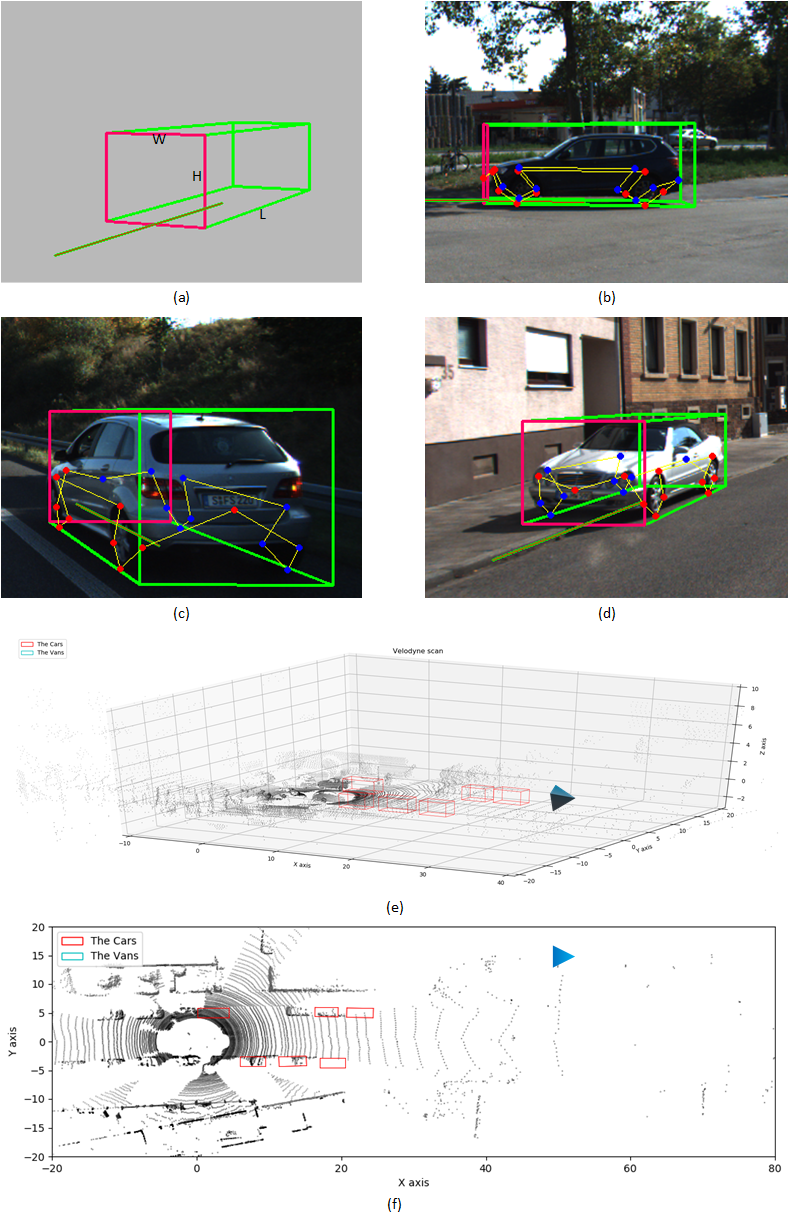
\includegraphics[width=1\textwidth]{visualization.png}
	\caption{Visualization of 3D bounding box and visibility. (a). visualization mechanism, (b). side view of visualization, (c). back view of visualization, (d). front view of visualization}
	\centering
	\label{figure:visualization}
\end{figure}







\section{Experiment and Evaluation}
In this section, we describe the experiment setup, discuss the most crucial design choices for our approach, evaluate our approach and its variations , and compare our approach with the start-of-the-art methods on monocular pose estimation of vehicles.  

template \tbd Experiments are divided into three parts1. First we compare with state-of-the-art methods for 3D object detection on KITTI [10] and SUN-RGBD [33] (Sec 5.1). Second, we provide in-depth analysis to validate our design choices (Sec 5.2). Last, we show qualitative results and discuss the strengths and limitations of our methods (Sec 5.3).

\subsection{Experiment Setup}

We have presented the approach in Section \ref{network} and \ref{inference} which is served as a baseline model of our approach. Some other design choices are made based on it. The benchmark network use ResNet50 \cite{DBLP:journals/corr/HeZRS15} as feature extractor, initialized with pre-trained weights trained on ImageNet \cite{DBLP:Russakovsky14}, and is trained with Adam \cite{DBLP:journals/corr/KingmaB14}. The network is implemented on Keras \cite{chollet2015keras} using TensorFlow \cite{tensorflow2015-whitepaper} as backend. Keras supports running both on GPU and CPU. 

We evaluate our approach and its variations on the dataset created based on KITTI 3D object detection benchmark \cite{Geiger2012CVPR}, described in Section \ref{data}. Because the KITTI only releases the ground truth for 7481 training images, we split them into train and validation set for training and validation respectively. We follow difficulty division policy of  KITTI and extend to more detailed levels \tbd. We use 54 vehicle CAD models \cite{NIPS2012_4562} for semi-automatic labelling and template matching. Each model is encoded with 20 points for its corresponding 3D sketch.

We evaluate six tasks: 3D vehicle detection, orientation estimation, 3D localization, 3D dimension estimation, 2D part localization, and 2D part visibility prediction. 3D vehicle detection is the ultimate task, representing the localization, orientation, and dimension of 3D bounding box,  which is therefore used to evaluated all the design choices.
\subsection{Evaluation Metrics}

We use intersection over union (IoU) to measure the performance of 3D vehicle detection. IoU used to measure the similarity of two 2D bounding boxes in various 2D object detection challenges, \eg Pascal VOC \cite{Everingham15} and ILSVRC \cite{DBLP:Russakovsky14}. Recently it is extended to measure 3D object detection with the formula:
\begin{equation}
	IoU(b_1, b_2) = \frac{V(b_{pre}\cap b_{gt})}{V(b_{pre}\cup b_{gt})}
\end{equation}
where $V(\cdot)$ indicates the volume and $b_{pre}$ denotes the predicted 3D bounding box while $b_{gt}$ is the ground truth. KITTI 3D object detection benchmark considers that a 3D object detection is correct, if $IoU \geq 0.5$ \cite{Geiger2012CVPR}. If multiple bounding boxes are predicted for one vehicle, they are considered as false predictions. %{But in our experiment, we lower the criterion to $IoU \geq 0.5$.}% 

For 3D orientation estimation, we use the measure,Orientation Score (OS), defined in \cite{DBLP:journals/corr/MousavianAFK16}. It is the mean error across all estimations in the validation set, written as:
\begin{equation}
	OS =\frac{1}{N} \sum_{i=1}^N\frac{(1+\cos(\triangle \theta_i))}{2}
\end{equation}
where $N$ denotes the number of examples in the validation set and $\triangle \theta_i$ represents the difference between the predicted orientation $r_y$ and the ground truth for example $i$.

 For other tasks, We follow the metrics set by \cite{DBLP:journals/corr/ChabotCRTC17}. A 3D localization is considered correct if its distance to the ground truth is less than a threshold. Two thresholds, 1 meter and 2 meters, are chosen. 2D part localization are measured the same way and the threshold is 20 pixels. 3D dimension estimation is correct if the predicted dimensions $(h, w, l)$ satisfies the equation
\begin{equation}
	\left | \frac{h-h_{gt}}{h_{gt}} \right | < 0.2  ~~\&~~\left | \frac{w-w_{gt}}{w_{gt}} \right | < 0.2  ~~\&~~ \left | \frac{l-l_{gt}}{l_{gt}} \right | < 0.2
\end{equation}
where $(h_{gt}, w_{gt}, l_{gt})$ is the ground truth. 2D part visibility prediction is a pure classification problem so that the measure is the accuracy over 4 classes.

Mean distance error (MDE) \tbd

\renewcommand{\arraystretch}{1.5}
\begin{table}[ht]
	\centering
	\caption{Metrics for six tasks}
	\label{my-label}
	\begin{tabular}{|m{6cm}|m{6cm}|}
		\hline
		Task                    & Metric         \\ \hline
		3D vehicle detection    & $IoU \geq 0.5$ \\  \hline
		3D orientation estimation  & $OS$     \\ \hline
		3D localization         &$\bf \lVert \overline t_{pre} - \overline t_{gt} \rVert$ $< 1 / 2$ meters   \\ \hline
		3D dimension estimation & $\left | \frac{d-d_{gt}}{d_{gt}} \right | _{d =\{h,w,l\}}<  20\%$           \\ \hline
		2D part localization    & $ \bf \lVert \overline p_{pre} - \overline p_{gt} \rVert $$<  20$ pixels      \\ \hline
		2D part visibility      &     $V_{pre} = V_{gt}$         \\ \hline
	\end{tabular}
\end{table}

\include{comparison}

\section{Conclusion and Discussion}
\subsection{Discussion}
In this section, we discuss the deficiencies of our approach, analyse their causes and propose some possible improvements.

\subsubsection{Deficiency of 2D Coordinate Labelling}
\label{2d_def}
\paragraph{Deficiency of Our Labelling Approach}
Our approach requires accurate 2D characteristic points to perform 2D-3D matching to calculate the location and orientation of the vehicles. However precisely labelling these points is demanding or even impossible for some vehicles with our semi-automatic labelling tool. The deficiency of labelling results from our labelling approach and the KITTI dataset.

Due to the variety of dimensions and shapes of vehicles, it is very hard to find a model that exactly matches the target vehicle with a small set of models. But if we expand the model set to cover all vehicles, the required quantity is too huge to satisfy. Therefore, we can only use a small set of models which means that the approximation and scaling are inevitable. And this will introduce errors to the labelling of 2D coordinates. Figure \ref{figure:label_def} (a) and (b) show two bad labelled examples. The imprecision of (a) results from the approximation of model matching, \ie most points are labelled correctly but point 1-6 are not. This is because the model can't perfectly fit the vehicle. The wrongly labelled points around wheels roots in the scaling the model to fit the vehicle so that, for example, the distance between point 4 and 8 are larger than the diameter of the wheel. The other pairs of points around the wheel have similar situation so that most points are not labelled correctly for this vehicle.

\begin{figure}[H]		
	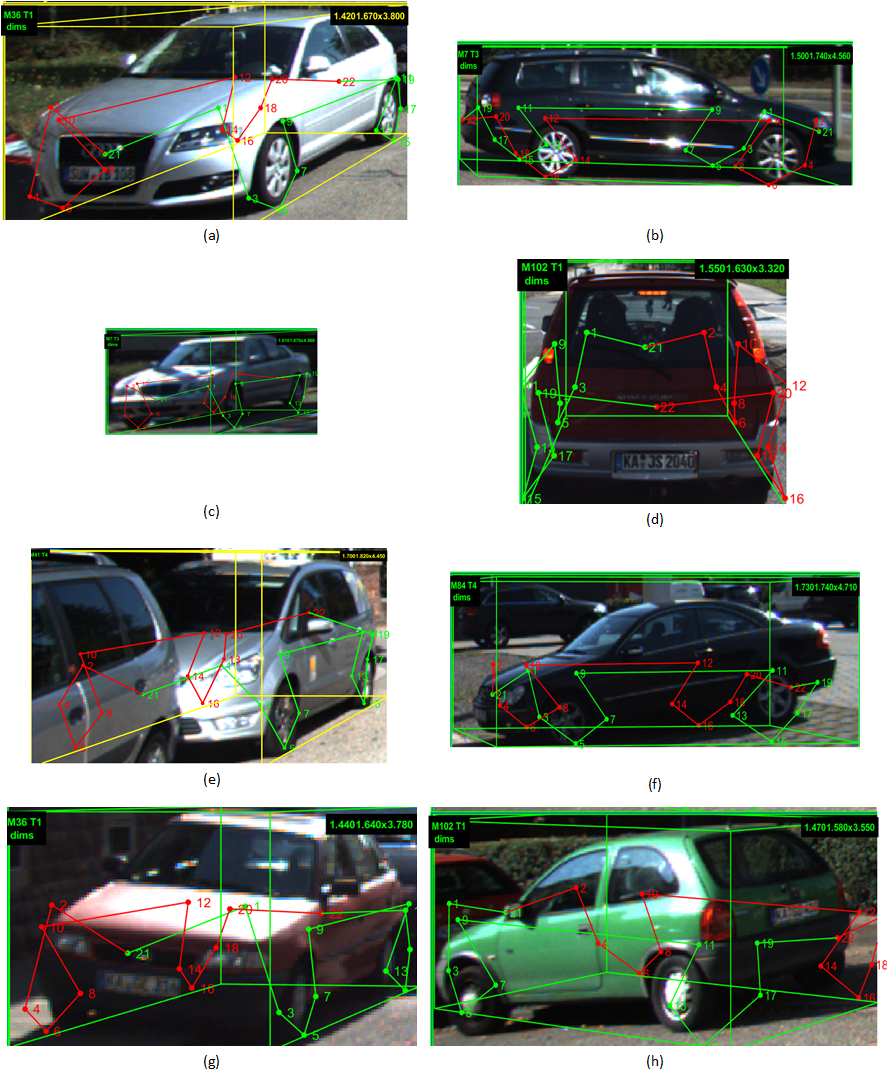
\includegraphics[width=0.8\textwidth]{label_def.png}
	\caption{Labelling examples for 2D points with original size. (a). Approximation results in inaccurate label for point 1-6. (b). Scaling change the relative distance between points which lead to bad labelling for points around the wheels. (c). One of the very small vehicles in image is able to be labelled with our approach. (d). The example that the side faces are not visible is able to be labelled with our approach. (e). The occluded vehicle can also be labelled with our approach. (f). The 3D bounding box ground truth of this vehicle is not correctly labelled in KITTI dataset. (g). KITTI doesn't consider the rotation along the roll axis, which results in bad labelling. (h). KITTI doesn't consider the rotation along the pitch axis, which results in totally wrong labelling.}
	\centering
	\label{figure:label_def}
\end{figure}

\paragraph{Deficiency of KITTI Dataset Labelling}
Our labelling approach requires very accurate label of the dataset because 2D points are very sensitive to the exact location of the target vehicle. But some of the KITTI images are not labelled so well that our approach makes mistakes. There are three main deficiencies of the KITTI labelling as shown in Figure \ref{figure:label_def} (f), (g), and (h). (f) shows the 3D bounding box ground truth of this vehicle is not correctly labelled. The 3D bounding box doesn't encompass the vehicle, especially the rear part, which leads to wrong labelling. (g) and (h) shows that our approach wrong labels the 2D points due to the assumption of KITTI that the vehicle only rotate along the yaw axis rather than the roll and pitch axis.


\paragraph{Possible Improvements}
Despite the drawbacks of our labelling approach, it has still has some advantages. Our approach can label very small vehicles in the image as shown in Figure \ref{figure:label_def} (c). Besides, it can label the self-occluded points as in Figure \ref{figure:label_def} (d) and the occluded and truncated points in Figure \ref{figure:label_def} (e). 

Therefore, if labelling labour is allowed, we can manually label the visible points for big vehicles and use the projection property and the geometry constraints to automatically generate the corresponding points. Therefore we have more accurate points for big vehicles. And for small and highly occluded or truncated vehicles, it is suitable to use our approach to label them. Because manually labelling these special vehicles is almost impossible and the error of our labelling approach can be decreased due to the quantities.


\subsubsection{Deficiency of Visibility Labelling}
\paragraph{Deficiency of Our Labelling Approach}
As described in Section \ref{visibility}, we label the visibility property of characteristic points with the help of the rotation $r_y$, other labelled objects, and the size of images. But there are two main shortcomings. The first one is that the 2D bounding box of a vehicle is larger in image than its real shape which makes our approach mistake the visible or self-occlude points as occluded. Figure \ref{figure:visib_def} (a). shows an example of labelling the self-occluded points as occluded, which leads to wrong labels. Another shortcoming is that our approach can't take the unlabelled objects into consideration so that it automatically ignores than during labelling. Figure \ref{figure:visib_def} (b) and (c) show two examples for this case. Our approach can't consider the traffic sign in (b) and the building in (c) and thus, it fails to label these occluded points correctly.

\begin{figure}[H]		
	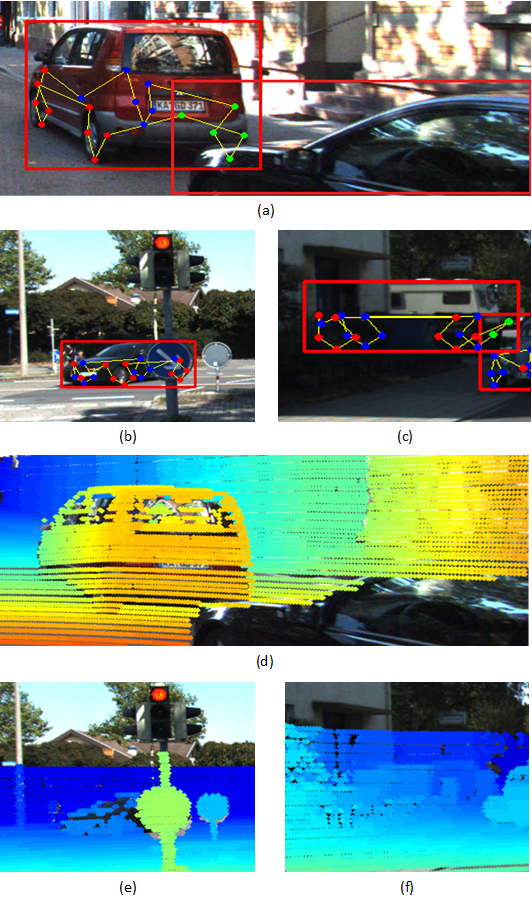
\includegraphics[width=0.7\textwidth]{visib_def.png}
	\caption{Labelling examples for visibility with original size. (a). The 2D bounding box is larger than the vehicle's real size, which results in labelling the self-occluded points as occluded. (b). KITTI doesn't label the traffic sign so that our approach can't label the occluded points correctly. (c). KITTI doesn't label the building so that our approach can't label the occluded points correctly.}
	\centering
	\label{figure:visib_def}
\end{figure}

\paragraph{Possible Improvements}

KITTI offers the LiDAR data for all images, which can provide the depth information of each pixel point in image or at least of a very small region. And based on the ground truth of location, orientation, and dimension of vehicles given by KITTI, we can calculate the depth of points distributed on the surface of the vehicles. By comparing these two kinds of depth information, we can correctly figure out whether there is some object in front of the target vehicle or not and which parts of the target vehicle are occluded, and thus we can classify the visibility properties correctly. Figure \ref{figure:visib_def_lidar} shows the images with LiDAR projection for examples in Figure \ref{figure:visib_def}. With the LiDAR depth information, we can easily classify the points around rear in (a) as self-occluded, and the occluded objects in (b) and (c) can be clearly detected and thus, we can assign the points whose depth is deeper than these objects as occluded. Therefore, for more accurate visibility labelling, it is worth making use of the LiDAR data.

\begin{figure}[H]		
	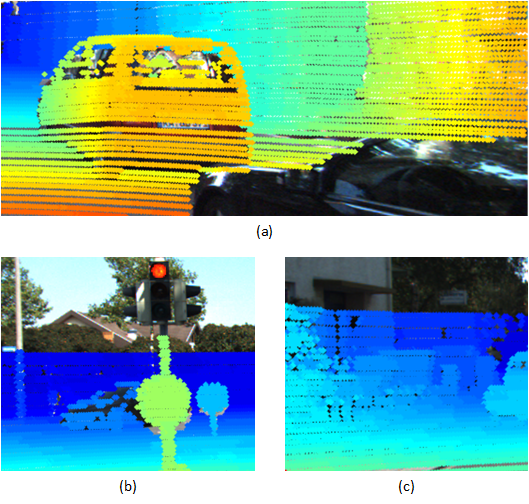
\includegraphics[width=0.7\textwidth]{visib_def_lidar.png}
	\caption{Images with LiDAR data projection for examples in Figure \ref{figure:visib_def} (a), (b), and (c) respectively.}
	\centering
	\label{figure:visib_def_lidar}
\end{figure}

\subsubsection{Deficiency of Template Matching}
In our approach, there are two situations where template matching is performed to fit a target vehicle with a 3D vehicle model. The first one is during labelling, when a 3D vehicle sketch is required to be projected into the KITTI images to generate 2D coordinates of key points for a target vehicle. And the model is selected via dimension matching. Another is during inference phase, where one 3D sketch is needed to generate the corresponding 3D coordinates of the key points for the target vehicle in the world coordinate system. The time the model is selected based on the estimated template proximity vector, \ie the ratios of 3 dimensions between the target vehicle and all 3D vehicle models.

For both cases, the most fundamental drawback is that we can only match the target vehicle with an approximate model based on the Dims strategy. This would results in errors in 2D and 3D coordinates of key points and thus impacts the final 3D vehicle pose estimation.

\paragraph{Possible Improvements}
As we mentioned before, the geometric property of 3D sketch relies heavily on the type of the vehicles. Therefore, a possible improvement for matching is to introduce type information into the matching phase. And there are some out-off-shelf frameworks can provide this kind of information \cite{DBLP:journals/corr/YangLLT15, 7780697, 7410527, DBLP:journals/corr/DehghanMSO17}, \ie Afshin \etal provide a network can recognize the Make and Model of vehicles \cite{DBLP:journals/corr/DehghanMSO17}. 

In sum, the optimal matching strategy is we first collect a 3D vehicle dataset where the distribution of vehicle dimensions covers the main part of the distribution of real vehicle dimensions in a fine-grained style, and during the matching, we first estimate the type of the vehicle and then select the best model via dimension matching from the same category. 

\subsubsection{Deficiency of Whole Approach}
The first unpleasant thing of this approach is the additional labelling work. This is so time consuming that it takes more than two month to find a proper method to generate the additional labels at an acceptable accuracy level. Besides, even with this method, the accuracy of the labels is compromised.

Moreover, our approach requires an additional 3D vehicle model dataset to encode the geometry information of vehicles, which makes it hard to generalize to vehicles without a corresponding model in the model dataset. For example, our approach can't perform accurate 3D pose estimation of buses because we don't include the bus models.

According to the competition results of KITTI 3D object detection, the approach that relies on single sensor can't compare with those making use of multi-sensor data \cite{3dobject}. RGB images captured by cameras have high resolution and good texture knowledge but lack depth information, which cloud points collected by LiDAR have 3D information of the scene but the resolution is relative lower and lack texture information. Therefore we think the best performance would be achieved by some approach driven by sensor fusion. If we have can start this task again, this is the first direction we will explore.






 \subsection{Conclusion}
 This thesis deals with the problem of 3D pose estimation of vehicles based on monocular images by using deep neural networks for the application of autonomous driving. Our approach can simultaneously performs 3D vehicle detection, 3D localization, 3D orientation estimation, 3D dimension estimation, 2D part localization, and parts visibility characterization for a vehicle in a 2D bounding box patch. It achieves state-of-the-art performance on six tasks. \tbd

\bibliographystyle{plain}
\bibliography{reference}
%\printbibliography

\end{document}